\chapter{Body of Argument}
\section{Intrinsic Motivation Inventory}
For this exam, the following question has been chosen to examine:

\begin{fancyquotes}
Question 6: Flow State and Intrinsic Motivation Inventory Questionnaires
Design a set of questions based on Flow State and Intrinsic Motivation Inventory Questionnaires for your project/larger project as discussed in Lecture 8.

Discuss the potential cross-overs of the two systems with the items you have chosen, the rationales behind the chosen items and the process for customization of the items to address the identified queries for your own project. Implement and/or design an experimental future set up for your project where you would implement these questionnaires and discuss expected/actual outcomes. 

\end{fancyquotes}

For this task, a paper entitled \textit{Intrinsic Motivation Inventory (IMI)} has been provided. It's a multidimensional measurement device that can be used to assess participants' subjective experience related to a target activity in laboratory experiments \citep{imiOne}. The paper will form the basis for the questionnaires that will be formulated in regards to our group's project.

According to \cite{imiTwo}, the intrinsic motivation inventory has gained widespread acceptance as a way to measure intrinsic motivation in the context of sport and exercise. It determines an individual's level of intrinsic motivation as an additive function of a set of underlying dimensions. It assesses participants' \textit{interest/enjoyment}, \textit{perceived competence}, \textit{effort}, \textit{value/usefulness}, \textit{felt pressure and tension} and \textit{perceived choice}, while performing a given activity. The interest/enjoyment subscale is deemed to be the most important, since it deals directly with intrinsic motivation \citep{imiOne}.

The IMI model consists of a big number of questions; however, the full set is rarely used, and it seems that inclusion/exclusion of any one factor does not affect the properties of the remaining factors \citep{imiTwo}. They can easily be modified to suit a specific activity \citep{imiOne}. E.g., an item such as "I tried very hard to do well at this activity" can be modified to a specific context, for instance a videogame, where it is replaced with "I tried very hard to do well on these puzzles in level 2".

\section{Designing Questionnaire For Extended Project} \label{qustionnaire}
For the extended project, a questionnaire was designed in order to gather information about the test participant's experience with the prototype developed during the course (see Figure \ref{fig:prototype}). The prototype consisted of a simple platforming game based around three different modalities: eye-tracking, accelerometer, posture/voice analysis.

\begin{figure}[htbp]
\centering
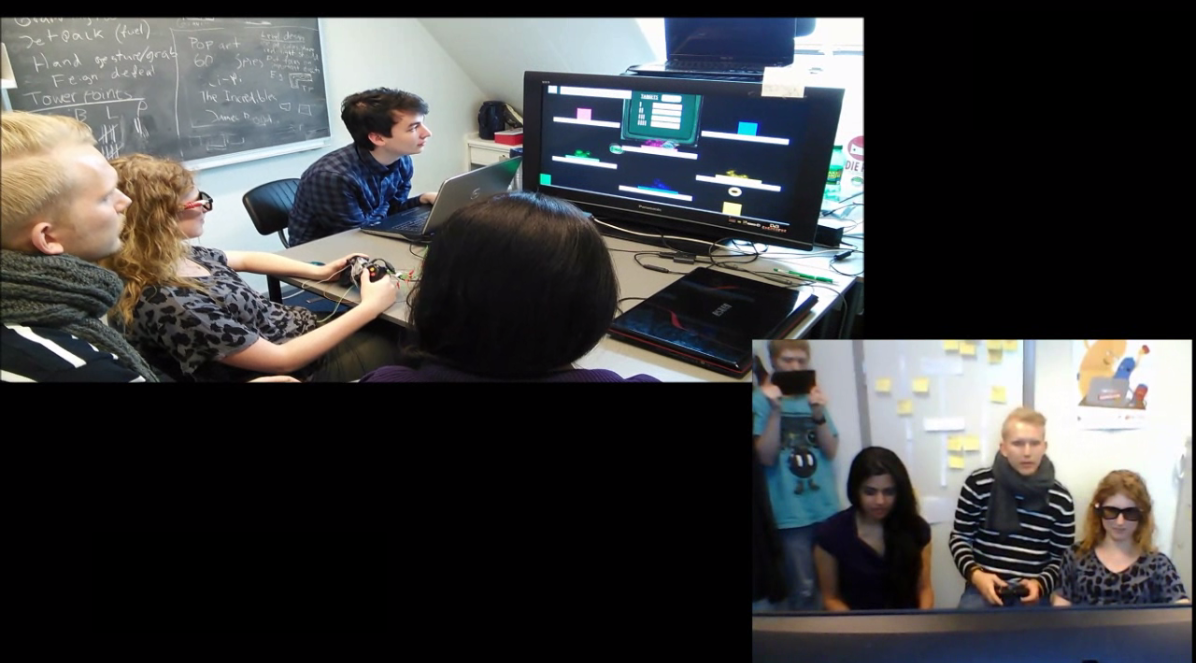
\includegraphics[width=0.70\textwidth]{Pictures/extended_modality}
\caption{Three test participants playing the prototype with extended modalities.}
\label{fig:prototype}
\end{figure}

Since it was a multiplayer game, one key area to explore was how participants felt in relation to each other. The social aspect was important, as well as players feeling engaged with the game, i.e., being in a flow-like state. Therefore, a set of questions were designed to gain insights in the participants experience with the game. These have been based on \cite{imiOne}, although with slight modifications.

\subsection{Questions Related to Flow}
For each question, participants were asked to rate themselves on a scale from 1 to 5, where 1 was "strongly disagree" and 5 was "strongly agree". For the sake of readability, the questions have here been ordered by the characteristics mentioned in Section \ref{char}. In the actual questionnaire, they were ordered randomly and without the headlines as shown in bold. Afterwards, a short description for each of the questions will be made.

%\begin{enumerate}
%\item I knew clearly what I wanted to do.
%\item It was really clear to me how my performance was going.
%\item My abilities matched the high challenge of the mission.
%\item I had a strong sense of what I wanted to do.
%\item It was no effort to keep my mind on what was happening.
%\item I was not concerned with how others may have been evaluating me. 
%\item I loved the feeling of the mission and want to capture it again.
%\item The challenge and skills among other players were at an equally high level.
%\item I did things spontaneously and automatically without having to think.
%\item My goals were clearly defined.
%\item I was completely focused on the task at hand.
%\item I found the experience extremely rewarding.
%\end{enumerate}
%1+2+4+10: clear goals and immediate feedback
%3: balance between skill/challenge
%5+11: present moment
%6: loss of oneself as social actor
%7+12: activity intrisic rewarding; want to do again
%8: balance between skill/challenge among other players, try to measure their flow states
%9: merging of action and awareness: just doing things automatically

\renewcommand{\labelenumiii}{\Roman{enumii}}
\begin{enumerate}
   \item \textbf{Intense and focused concentration on the present moment}
   \begin{enumerate}
     \item It was no effort to keep my mind on what was happening
     \item I was completely focused on the task at hand
   \end{enumerate}
   \item \textbf{Merging of action and awareness}
   \begin{enumerate}
     \item I did things spontaneously and automatically without having to think
   \end{enumerate}
   \item \textbf{Loss of reflective self-consciousness (loss of awareness of oneself as a social actor)}
   \begin{enumerate}
     \item I was not concerned with how others may have been evaluating me
   \end{enumerate}
   \item \textbf{A sense that one can control one's actions}
   \begin{enumerate}
     \item My abilities matched the high challenge of the mission
     \item I knew clearly what I wanted to do
	 \item It was really clear to me how my performance was going
	 \item I had a strong sense of what I wanted to do
	 \item My goals were clearly defined
	 \item The challenge and skills among other players were at an equally high level
   \end{enumerate}
   \item \textbf{Distortion of temporal experience}
   \begin{enumerate}
     \item Time seemed to pass away very quickly
   \end{enumerate}
   \item \textbf{Experience of the activity as intrinsically rewarding}
   \begin{enumerate}
     \item I loved the feeling of the mission and want to capture it again
     \item I found the experience extremely rewarding
   \end{enumerate}
\end{enumerate}

For the first category about focus and concentration, it was chosen not to have too many questions, since it was deemed unrealistic to achieve an intense focus when testing the prototype. This was because of the state of the game, together with the additional modalities, being a mix of a rough prototype and a simple Wizard of Oz \citep{InteractDesign}. There were a lot of minor nuisance factors (such as participants having to wear sunglasses in order to simulate an eye-tracking system), which made it hard to concentrate fully on the game. Also, due to an accelerometer and Arduino board being taped to the participants' game controllers, movement were restricted because of short cords.

The second category set out to investigate to what extend participants acted without thinking. However, due to the nature of the prototype, a lot of elements weren't made totally clear, which meant that a facilitator had to instruct and/or help participants.

For the third category, loss of reflective self-consciousness, it was important to examine how concerned the participants were with each other. Since multiplayer games emphasize social interactions, this was an important question to ask. However, it is not enough just to get a rating, since it doesn't say anything about whether being concerned is a positive or negative thing. Some might like the attention of their peers, while others might not. Therefore, a comment field was introduced, so participants could give details on this question.

As mentioned several times, flow is about finding the balance between challenge and skills. This is why the fourth category multiple questions to examine this area. Additionally, it is important that the participants' goals were well-defined. Feedback should also be immediate and clear.

For the fifth category, one question was asked to gain insights on if participants felt that they lost their notion of time. However, since each test session lasted for less than 10 minutes, not a lot of effort was put into this category.

For the last category, two questions were asked about intrinsic motivation. It should be noted that the test participants didn't voluntarily ask to take part in the test. Instead, they might have felt a minor pressure to participate. This can have had an influence in their intrinsic motivation. Also, this area will be examined further in the following questions concerning intrinsic motivation.

\subsection{Questions Related to Intrinsic Motivation}
For the IMI part, a selection of questions were asked. Again, participants rated themselves on a scale from 1 to 5, where 1 was "strongly disagree" and 5 was "strongly agree".

\begin{enumerate}
\item I think I did pretty well at this activity, compared to other players
\item This was an activity that I couldn't do very well
\item I felt more close to the other players after playing the game
\item I put a lot of effort into this
\item I felt like I had choice about interacting with other players
\item I felt pressured while doing the activities
\item I trusted people less after playing the game
\item I felt like it was not my own choice to do the activities
\item I did not feel at all nervous about interacting with other players
\end{enumerate}

These questions are a little more varied, with the goal of examining the test participants' overall experience with playing the game. Compared to the previous flow-related questions that focused on one's personal experience (looking inwards), the IMI questions have more focus on player-to-player interaction (looking outwards). Since the context is a multiplayer game, it was important to investigate how the players feel about each other. Despite it being a competitive game where the goal is to beat the other players, it's also a social game where people, hopefully, bond with each other and feel more connected after playing. This is why the questions ask players about topics such as \textit{interacting with other players}, \textit{feeling more close after playing the game} and \textit{trusting players less after playing the game}. The last question was asked, since for the full project (that was going to be developed after this prototype), the game would be based on deceptive mechanics similar to bluffing in the game of poker.